\chapter{Ergebnis}\label{chap:experiments}

Nach der Beschreibung des Konzepts und Verlauf des Python-Skripts geht dieses Kapitel auf einige Trainingsdurchläufe ein  und diskutiert die Ergebnisse. 
\\\\
Es wurden iterativ Trainingprozeduren durchgeführt mit jeweils unterschiedlichen Konfiguration, wie im vorherigen Kapitel gezeigt, und miteinander verglichen. Die genauen Konfigurationen werden bei den einzelnen Experimenten angeführt. Die Experimente liefen auf einem Rechner mit NVIDIA TITAN Xp 12 GB VRAM Grafikkarte, Intel i7-7800X CPU und 32 GB RAM. Da diese Arbeit zeitlich begrenzt ist, wurden die Experimente auf max. 100 Epochen begrenzt, was die durchschnittliche Laufzeit auf etwa drei bis vier Stunden je Experiment bringt. Diese Beschränkung wirkt ebenfalls Overfitting entgegen, da das Modell nicht ausreichend Zeit hat, um sich auf den Trainingsdatensatz "`einzugewöhnen"'. Wobei sich dieser Zeitpunkt, wo ein Modell zu lange lernt, sich verschieben kann und von der untersuchten Problematik abhängig ist.
\\\\
Es wurden drei unterschiedliche Datensätze aus den Sentinelprodukten erzeugt. 
\begin{enumerate}
	\item Der originale unaugmentierte Datensatz enthält insgesamt jeweils zwölf Bilder und Masken\footnote{Trainingsanteil: 7, Validationsanteil: 2, Testanteil: 3} und dient als Basis für das Ausgangsexperiment. 
	\item Der augmentierte Datensatz (s. Kapitel \ref{sec:augmentation}) enthält 1291 Dateien und Masken\footnote{Trainingsanteil: 825, Validationsanteil: 207, Testanteil: 259}. Nachdem die zufällige Ausschnitte produziert wurde, kam es vor, dass einige Masken keinen \textit{RoI}-Anteil enthielten. Diese Masken und auch die zugehörigen Bilddateien wurden verworfen und der Datensatz weicht deswegen von der eigentlichen Größe von 1296 Elementen\footnote{Die zwölf ursprünglichen Dateien multipliziert mit dem Data Augmentation-Faktor von 108.} ab.
	\item In einem dritten Datensatz wurden Ausschnitte benutzt, deren Bildgrenzen sich an den äußersten Punkten der Masken befinden (s. Abb. \ref{fig:example-overfitting}). Dieser Datensatz wurde ausschließlich mittels Rotationen erweitert und enthält 144 Elemente\footnote{Trainingsanteil: 92, Validationsanteil: 23, Testanteil: 29}. 
\end{enumerate}
\noindent

\section{Training mit Rohdaten}\label{sub:sub:sec:experiment-1}

\begin{lstlisting}[language=python,caption={Konfiguration für Experimente 1},captionpos=b]
class CropDiseaseConfig(Config):
    BACKBONE = "resnet50"
    IMAGE_MAX_DIM = 128
    IMAGE_MIN_DIM = 128
    IMAGE_RESIZE_MODE = "square"
    IMAGES_PER_GPU = 4
    LEARNING_RATE = 0.001
    NUM_CLASSES = 1 + 1
    RPN_ANCHOR_SCALES = (8, 16, 32, 64, 128)
    STEPS_PER_EPOCH = 23
    USE_MINI_MASK = False
\end{lstlisting}
\noindent
Hier wurde Datensatz 1 benutzt und alle Schichten des Modells wurden trainiert. Diese Experimente sollen zeigen, wie ein zu kleiner Datensatz sich auswirken kann.

\begin{figure}[ht]
	\centering
    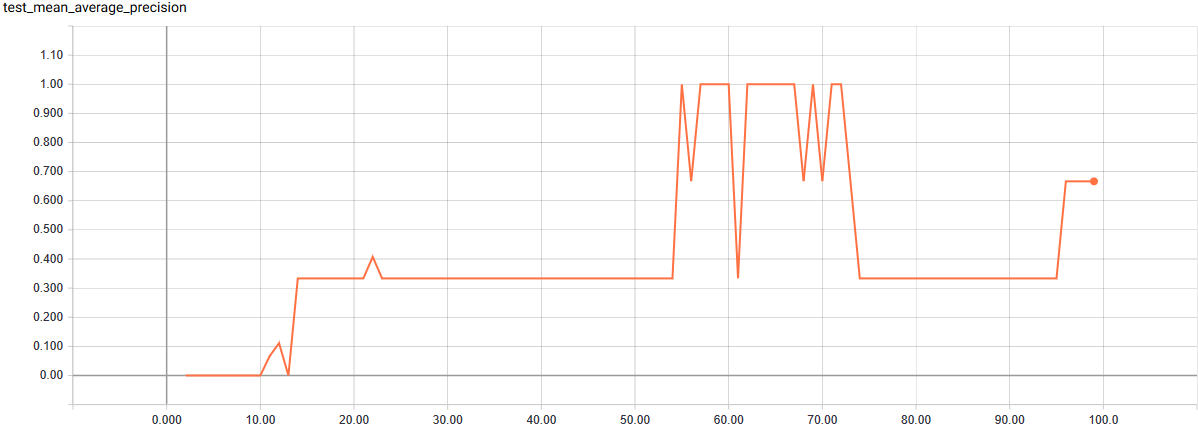
\includegraphics[width=.7\textwidth]{pics/map-1.PNG}
    \caption[\textit{mAP}-Graph von Experiment 1]{\textit{mAP}-Graph von Experiment 1, X-Achse: Epochennummer, Y-Achse: \textit{mAP}-Werte}
    \label{fig:map-1}
\end{figure}
\begin{figure}[ht]
	\centering
    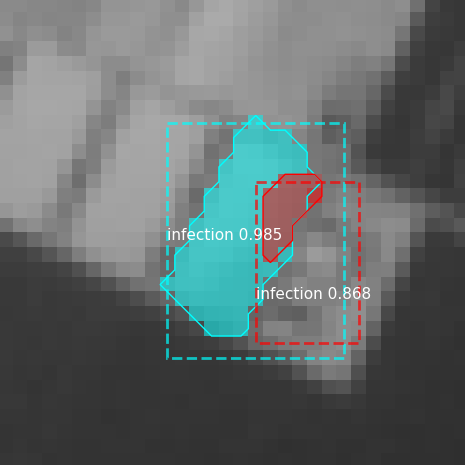
\includegraphics[height=3.5cm]{pics/pred-1-1.png}
    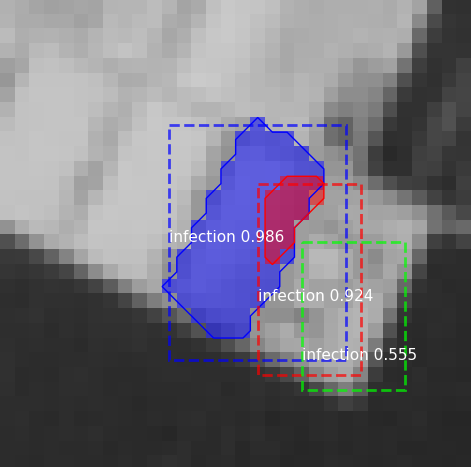
\includegraphics[height=3.5cm]{pics/pred-1-2.png}
    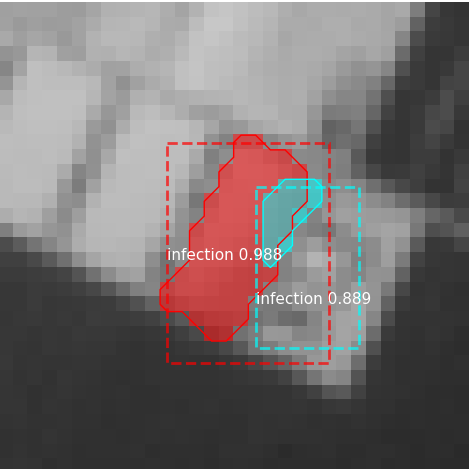
\includegraphics[height=3.5cm]{pics/pred-1-3.png}
    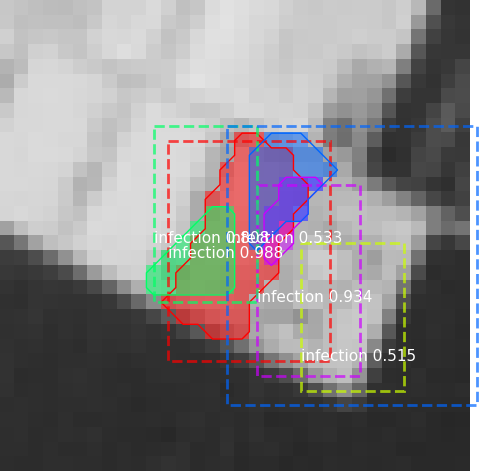
\includegraphics[height=3.5cm]{pics/pred-1-4.png}
    \caption[Beispielvorhersagen Experiment 1]{Beispielvorhersagen anhand der Gewichte von Epoche 55}
    \label{fig:pred-1}
\end{figure}
\noindent
Man sieht, dass das Modell während des Trainings unterdurchschnittliche Ergebnisse erzielt, was wenig überraschend ist, da der Datensatz sehr klein ist. Da nach jeder Epoche die Gewichte zwischengespeichert werden, können diese einzeln geladen werden. So wurde für eine Detektion ein Modell mit den Gewichten der 55. Epoche initialisiert, da sich hier der \textit{mAP}-Wert auf dem Maximalwert befindet. Die Bilder in Abb. \ref{fig:pred-1} entstammen einem fremden Datensatz, ähneln aber in den Grundcharakteristika dem eigentlichen Datensatz 1. Zum Beispiel ist das Zielfeld ähnlich ausgerichtet und zentriert. Man sieht, dass sich die berechneten Masken relativ genau auf das Zielfeld eingrenzen. Jedoch passen die erzeugten Bounding-Boxen nicht zu den entsprechenden Masken, falls eine Maske erkannt wurde. Auch wurden mehrere Objektinstanzen erkannt, wobei eine einzige Instanz detektiert werden sollte. Werden die Bilder in Abb. \ref{fig:pred-1} nun vertikal gespiegelt und in das Netzwerk gegeben, erzeugt das Modell keine Masken, obwohl lediglich die Ausrichtung verändert wurde. Das ist ein Hinweis auf Overfitting, da das neuronale Netz minimale Änderungen nicht mehr erkennt.

\section{Datensatzerweiterung durch Rotation}\label{sub:sub:sec:experiment-2}

\begin{lstlisting}[language=python,caption={Konfiguration für Experiment 2},captionpos=b]
class CropDiseaseConfig(Config):
    BACKBONE = "resnet50"
    IMAGE_MAX_DIM = 128
    IMAGE_MIN_DIM = 128
    IMAGE_RESIZE_MODE = "square"
    IMAGES_PER_GPU = 4
    LEARNING_RATE = 0.001
    NUM_CLASSES = 1 + 1
    RPN_ANCHOR_SCALES = (8, 16, 32, 64, 128)
    STEPS_PER_EPOCH = 206
    USE_MINI_MASK = False
\end{lstlisting}
\noindent
Bei diesem Experiment wurde ein Modell Datensatz 3 und alle Schichten des Modells trainiert. Die Konfiguration bleibt unverändert, jedoch ist hier der augmentierte Datensatz vergleichsweise größer.

\begin{figure}[ht]
	\centering
    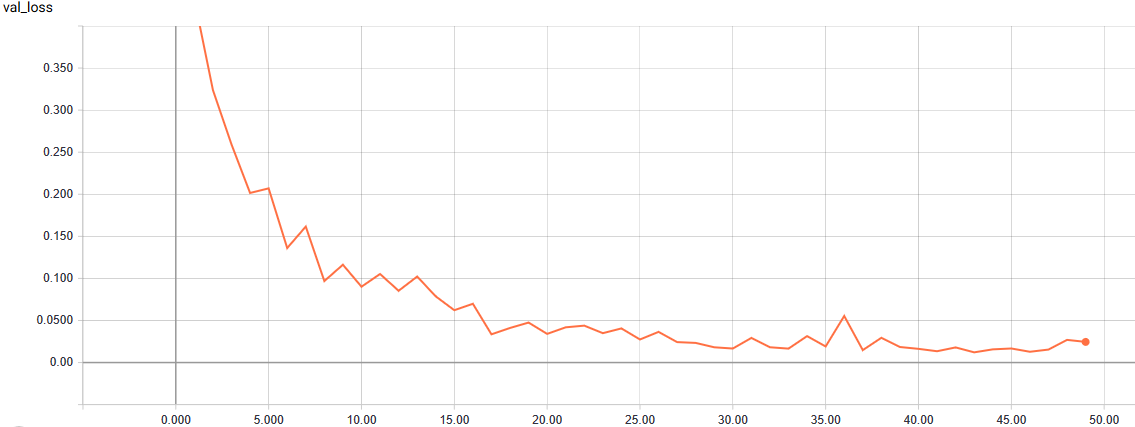
\includegraphics[width=.7\textwidth]{pics/val-loss-2.PNG}
    \caption[\textit{loss}-Graph von Experiment 2]{\textit{loss}-Graph von Experiment 2, X-Achse: Epochennummer, Y-Achse: \textit{loss}-Werte}
    \label{fig:val-loss-2}
\end{figure}

\begin{figure}[ht]
	\centering
    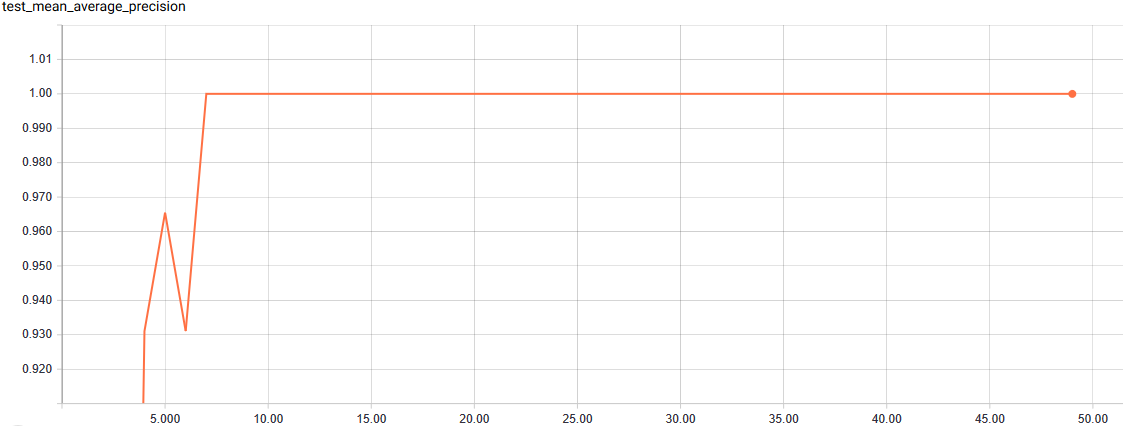
\includegraphics[width=.7\textwidth]{pics/map-2.PNG}
    \caption[\textit{mAP}-Graph von Experiment 2]{\textit{mAP}-Graph von Experiment 2, X-Achse: Epochennummer, Y-Achse: \textit{mAP}-Werte}
    \label{fig:map-2}
\end{figure}

\begin{figure}[ht]
  \centering
  \begin{minipage}[c]{.3\textwidth}
  \centering
  
\includegraphics[height=2cm]{pics/roi-2-1.png}
  \\ \vspace{.25cm}
  
\includegraphics[height=3cm]{pics/roi-2-2.png}
  \\ \vspace{.25cm}
  
\includegraphics[height=3cm]{pics/roi-2-3.png}
  \\ \vspace{.25cm}
  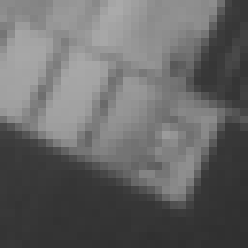
\includegraphics[height=3cm]{pics/roi-2-4.png}
  \end{minipage}
  \begin{minipage}[c]{.3\textwidth}
  \centering
  
\includegraphics[height=2cm]{pics/mask-2-1.png}
  \\ \vspace{.25cm}
  
\includegraphics[height=3cm]{pics/mask-2-2.png}
  \\ \vspace{.25cm}
  
\includegraphics[height=3cm]{pics/mask-2-3.png}
  \\ \vspace{.25cm}
  
\includegraphics[height=3cm]{pics/mask-2-4.png}
  \end{minipage}
  \begin{minipage}[c]{.3\textwidth}
  \centering
  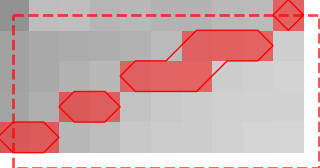
\includegraphics[height=2cm]{pics/pred-2-1.png}
  \\ \vspace{.25cm}
  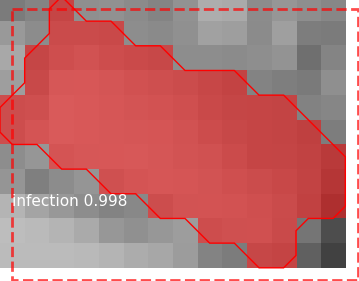
\includegraphics[height=3cm]{pics/pred-2-2.png}
  \\ \vspace{.25cm}
  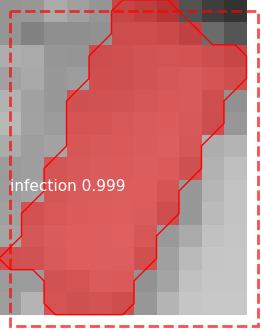
\includegraphics[height=3cm]{pics/pred-2-3.png}
  \\ \vspace{.25cm}
  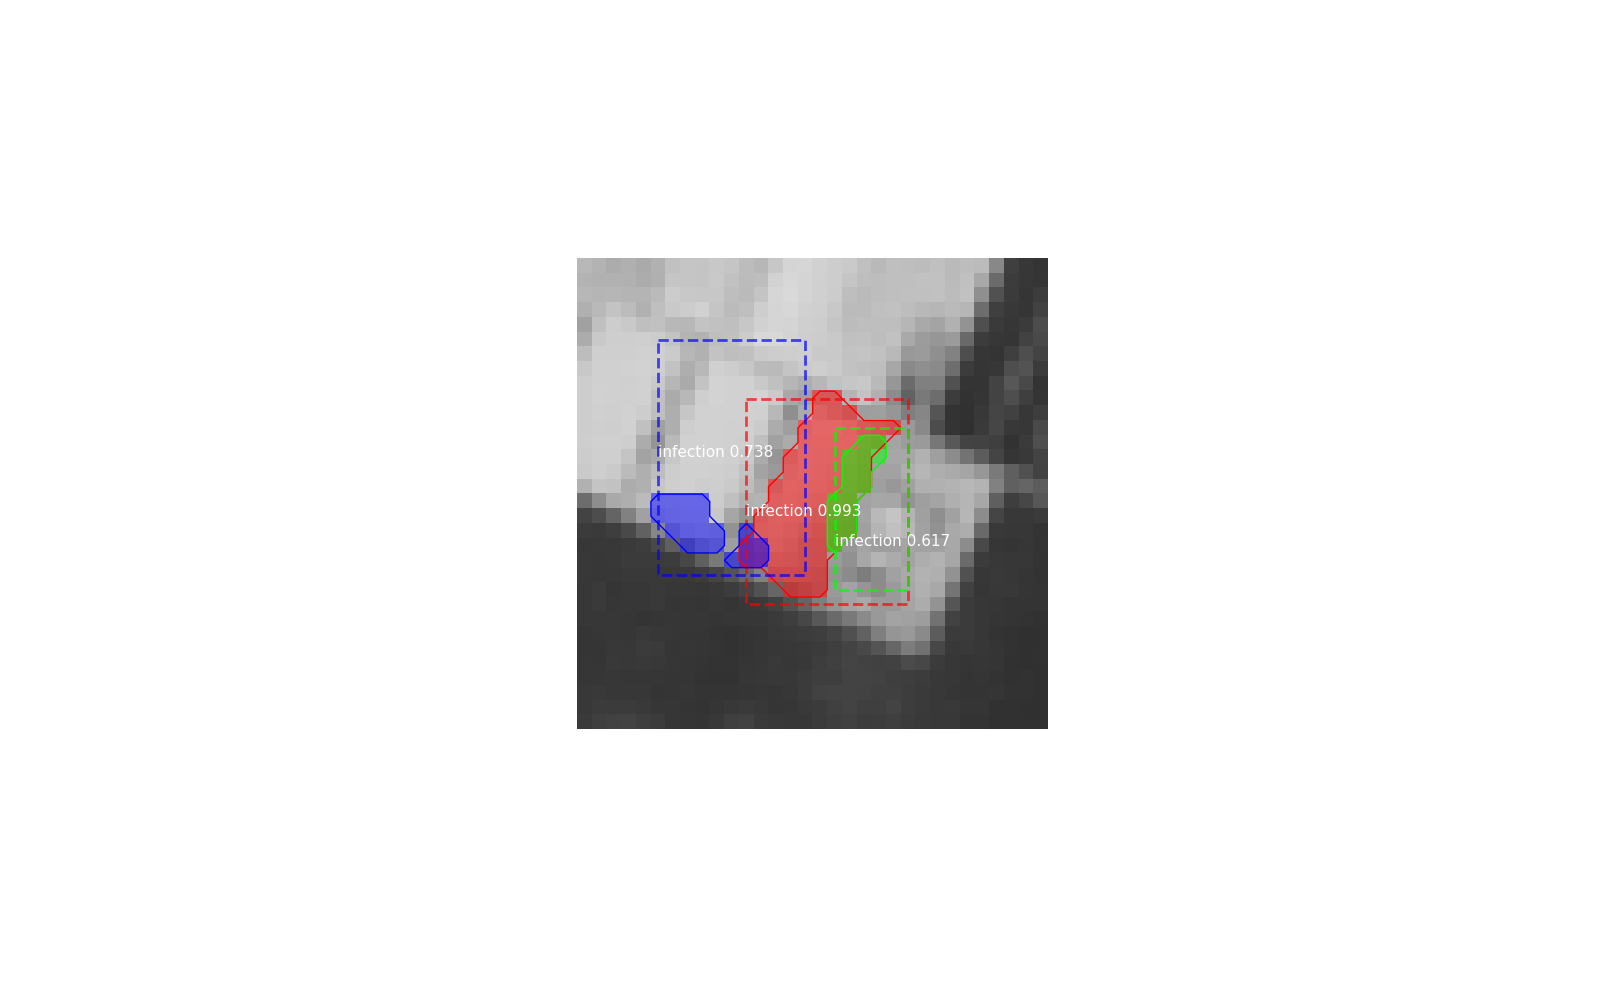
\includegraphics[height=3cm]{pics/pred-2-4.png}
  \end{minipage}

  \caption[Beispielvorhersagen Experiment 2]{Beispielvorhersagen anhand der Gewichte von Epoche 37, links: Ausgangsbild, mitte: Maske, rechts: Detektion}
  \label{fig:pred-2}
\end{figure}
\noindent
Die \textit{mAP}-Kurve konvergiert ab Epoche 7 gegen $1$ und verweilt dort für den Rest des Trainings. Dagegen sinken die $loss$-Werte weiterhin und nähern sich ab Epoche 37 $0$ an. Daher wurden die Gewichte dieser Epoche näher untersucht. Abb. \ref{fig:pred-2} zeigt, dass das Modell resistenter gegenüber Rotationen ist. Nichtsdestotrotz reagiert das Modell empfindlich auf Veränderungen wie zum Beispiel ein größerer Ausschnitt oder Translationen (s. unterste Reihe in Abb. \ref{fig:pred-2}). Daraus ergibt sich, dass das Modell nicht allgemein einsetzbar ist und die Daten durch weitere Augmentationen randomisiert werden müssen.
\newpage
\section{Data Augmention und Regularization}\label{sec:experiment-3}

\begin{lstlisting}[language=python,caption={Konfiguration für Experiment 3},captionpos=b,label=lst:experiment-3]
class CropDiseaseConfig(Config):
    BACKBONE = "resnet50"
    IMAGE_MAX_DIM = 128
    IMAGE_MIN_DIM = 128
    IMAGE_RESIZE_MODE = "square"
    IMAGES_PER_GPU = 4
    LEARNING_RATE = 0.001
    NUM_CLASSES = 1 + 1
    RPN_ANCHOR_SCALES = (8, 16, 32, 64, 128)
    STEPS_PER_EPOCH = 3
    USE_MINI_MASK = False
    WEIGHT_DECAY = 0.0001 # Orange, Dunkelblau, Rot
    WEIGHT_DECAY = 0.001 # Pink
    WEIGHT_DECAY = 0.01 # Hellblau
\end{lstlisting}

\noindent
Diese Sektion vergleicht mehrere Traingsläufe direkt miteinander. Zur simpleren Kommunikation werden die einzelnen Durchläufe mit den Farben betitelt, wie sie in den Graphen \ref{fig:val-loss-3} und \ref{fig:map-3} (Orange, Rot, Pink, Hell- und Dunkelblau) repräsentiert sind. Die verschiedenen \texttt{WEIGHT\_DECAY}-Werte in Listing \ref{lst:experiment-3} wurden in den entsprechenden Modellkonfigurationen verwendet, wie sie in den Kommentaren benannt sind, wobei der Wert für die orangene, rote und dunkelblaue Konfiguration implizit in der Basisklasse \texttt{Config} definiert ist. Die pinke und hellblaue Konfiguration soll den Einfluss von L2 Regularization zeigen. Alle Modelle bis auf das orangene wurden auf Grundlage von Datensatz 2 trainiert. Aus Gründen, die später erklärt werden, wurde für das orangene Modell ein Datensatz kreiert, der sich auf die kleine Zone innerhalb des Feldes mit der stärkeren Infektionskonzentration beschränkt. Der \textit{head} des dunkelblauen Netzwerk wurde trainiert, während alle Schichten der restlichen Modelle trainiert wurden.

\begin{figure}[ht]
	\centering
    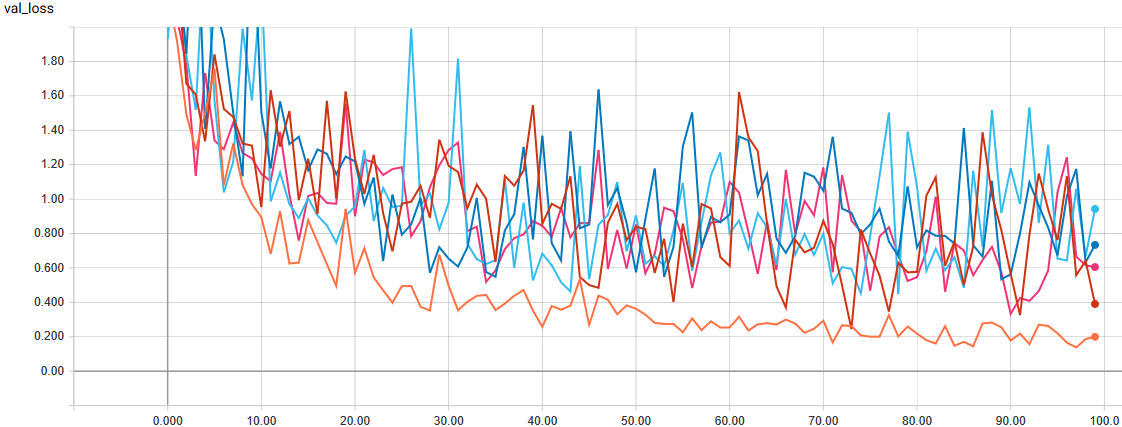
\includegraphics[width=.7\textwidth]{pics/val-loss-3.PNG}
    \caption[\textit{loss}-Graph von Experiment 3]{\textit{loss}-Graph von Experiment 3, X-Achse: Epochennummer, Y-Achse: \textit{loss}-Werte}
    \label{fig:val-loss-3}
\end{figure}

\begin{figure}[ht]
	\centering
    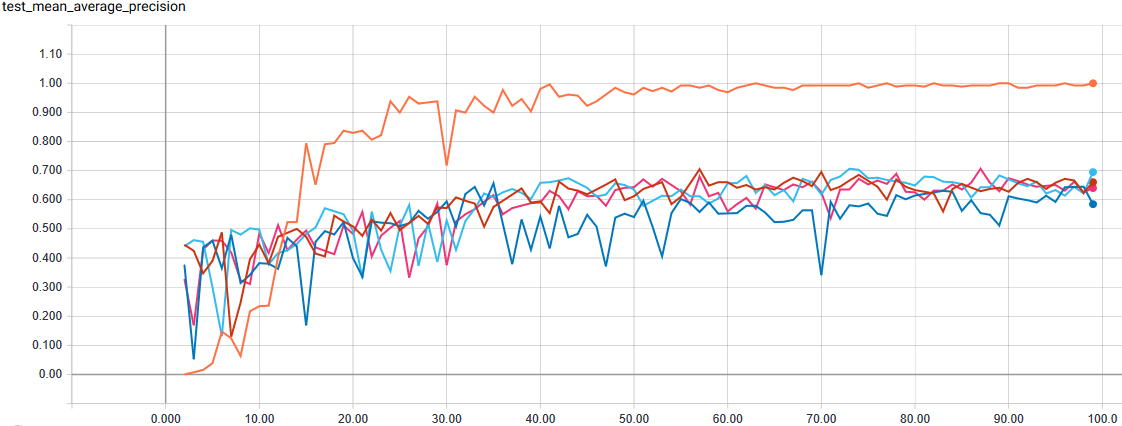
\includegraphics[width=.7\textwidth]{pics/map-3.PNG}
    \caption[\textit{mAP}-Graph von Experiment 3]{\textit{mAP}-Graph von Experiment 3, X-Achse: Epochennummer, Y-Achse: \textit{mAP}-Werte}
    \label{fig:map-3}
\end{figure}

\begin{figure}[H]
  \centering
  \begin{minipage}[c]{.3\textwidth}
  \centering
  
\includegraphics[height=3cm]{pics/roi-3-2.png}
  \\ \vspace{.25cm}
  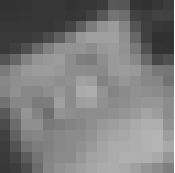
\includegraphics[height=3cm]{pics/roi-3-3.png}
  \\ \vspace{.25cm}
  
\includegraphics[height=3cm]{pics/roi-3-4.png}
  \\ \vspace{.25cm}
  
\includegraphics[height=3cm]{pics/roi-3-5.png}
  \\ \vspace{.25cm}
  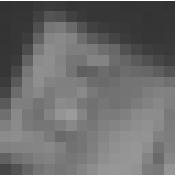
\includegraphics[height=3cm]{pics/roi-3-1.png}
  \end{minipage}
  \begin{minipage}[c]{.3\textwidth}
  \centering
  
\includegraphics[height=3cm]{pics/mask-3-2.png}
  \\ \vspace{.25cm}
  
\includegraphics[height=3cm]{pics/mask-3-3.png}
  \\ \vspace{.25cm}
  
\includegraphics[height=3cm]{pics/mask-3-4.png}
  \\ \vspace{.25cm}
  
\includegraphics[height=3cm]{pics/mask-3-5.png}
  \\ \vspace{.25cm}
  
\includegraphics[height=3cm]{pics/mask-3-1.png}
  \end{minipage}
  \begin{minipage}[c]{.3\textwidth}
  \centering
  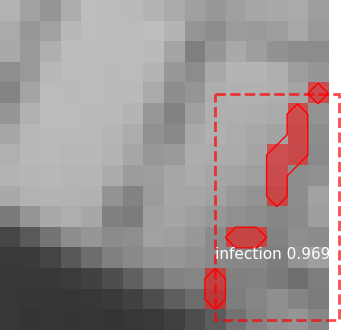
\includegraphics[height=3cm]{pics/pred-3-2.png}
  \\ \vspace{.25cm}
  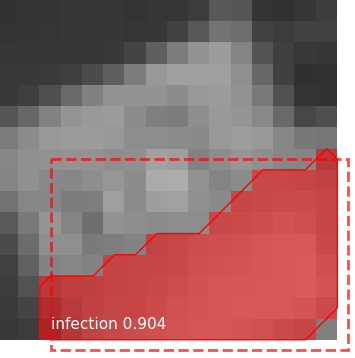
\includegraphics[height=3cm]{pics/pred-3-3.png}
  \\ \vspace{.25cm}
  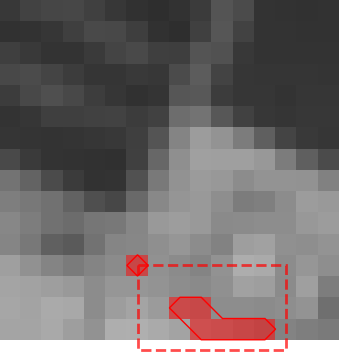
\includegraphics[height=3cm]{pics/pred-3-4.png}
  \\ \vspace{.25cm}
  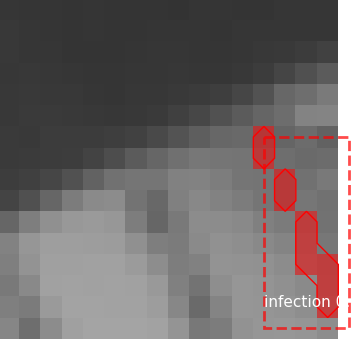
\includegraphics[height=3cm]{pics/pred-3-5.png}
  \\ \vspace{.25cm}
  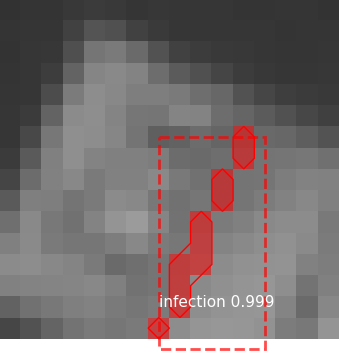
\includegraphics[height=3cm]{pics/pred-3-1.png}
  \end{minipage}

  \caption[Beispielvorhersagen Experiment 3]{Beispielvorhersagen verschiedener Modelle, v.l.n.r.: Ausgangsbild, Masken, Vorhersage, v.o.n.u.: Vorhersagen von dunkelblau, rot, hellblau, pink, orange}
  \label{fig:pred-3}
\end{figure}
\noindent
Für auf Datensatz 3 trainierte Modelle (jeweils Epoche 100) zeichnen sich in  Abb. \ref{fig:val-loss-3} starke Schwankungen ab und kein Modell überschreitet $mAP>0.7$. Die Vorhersagen in den oberen vier Reihen in Abb. \ref{fig:pred-3} stimmen zum großen Teil mit den Masken überein. Weitere hier nicht aufgeführte Vorhersagen zeigen ähnliche Ergebnisse. Es kommt vor, dass die kleine Zielregion vorhergesagt wird, obwohl die entsprechende binäre Maske die große \textit{RoI} repräsentiert, so ähnlich wie es in der unteren Reihe zu sehen ist. Dieses Verhalten erklärt die schlechten \textit{mAP}-Kurven und die Schwankungen. Da die Detektion nicht mit dem erwarteten Ergebnis übereinstimmt und daher der berechnete Fehler höher ist, obwohl die Detektion eigentlich korrekt ist, da sich beide genutzten \textit{RoIs} geografisch schneiden. Durch den Fehler ist die Korrektur der Gewichte entsprechend größer. Um die Annahme zu bekräftigen, wurde ein Modell (orange) auf dem speziellen Datensatz trainiert. Im Vergleich zu den anderen Kurven konvergiert die orangene \textit{loss}-Kurve gegen $0$ bzw. die orangene \textit{mAP}-Kurve gegen $1$. Wären mehrere unterschiedliche \textit{RoIs} vorhanden, die sich nicht schneiden, würde der Einfluss sich nicht bemerkbar machen. Was hier jedoch nicht der Fall ist, da beide \textit{RoIs} jeweils etwa die Hälfte des Datensatzes ausmachen.
\\\\
Es ist zu sehen, dass die \textit{Ridge Regression} (hellblau und pink) keinen merkbaren Einfluss auf das Training haben, weil sie einen ähnlichen Verlauf wie die dunkelblaue und rote Kurven haben. Im Gegensatz dazu zeigt die \textit{Data Augmentation} positive Ergebnisse (s. Abb. \ref{fig:pred-3}) und alle Modelle sind deutlich robuster gegenüber manipulierten Bildern. Jedoch schlagen die Detektionen bei größeren Ausschnitten fehl oder geben sinnlose Resultate zurück. Weiterhin sei erwähnt, dass das Modell, dessen \textit{head} trainiert wurde, von allen hier erwähnten Modellen am schlechtesten abschneidet und es zumindest nicht hilfreich ist, nur die oberen Schichten zu trainieren.

\section{Ergebnisdiskussion}

Ergebnisse zeigen, dass Mask R-CNN ein potentielles Werkzeug ist, um Landwirte bei der Kontrolle ihrer Felder zu unterstützen. Die implementierte Anwendung lädt automatisch Sentinelprodukte herunter, extrahiert die gefragten Bildregionen und berechnet daraus einen Gesundheitsindex der Flächen. Ein konfiguriertes Mask R-CNN-Modell analysiert die Indexwerte auf Muster, die mit Krankheiten korrelieren könnten. 
\\\\
Das Ziel der Arbeit, eine Vielzahl von Krankheiten zu analysieren und zu identifizieren, konnte nicht erreicht werden, da hier nur zwei Regionen zur Verfügung standen. Aufgrund dessen wurden wie erwartet bei ersten Experimenten Modelle trainiert, die Overfitting aufwiesen. Nichtsdestotrotz half Data Augmentation, die Größe des Datensatzes zu erweitern und Variationen in Form und Ausrichtung der Ausgangsfläche zu erzeugen. Dadurch konnte ein Modell trainiert werden, das Resistenz gegenüber Overfitting aufwies. Der Einsatz von Data Augmentation ist ebenfalls sinnvoll, sollte kein Overfitting vorliegen. Ausbreitungen von Infektionen sind willkürlich und folgen keinen bestimmten geometrischen Mustern. Data Augmentation hilft durch künstliche Randomisierungen ein Modell darauf vorzubereiten.
\\\\
Jedoch zeigte die oft bei Overfitting verwandte Ridge Regression keinerlei Auswirkung. Wenn einige ausgewählte Neuronen-Schichten trainiert wurden, verschlechterte sich die allgemeine Performanz. Deswegen sind L2 Regularization und Training ausgewählter Schichten in weiteren Untersuchungen, die nur mit hier untersuchten Felddaten arbeiten, nicht zu empfehlen. 
\\\\
Weiterhin wurde die Vermutung aufgestellt, dass die \textit{RoIs} negative Einflüsse auf die Bewertung des Trainings haben, da eine Region von der zweiten Region umschlossen wird. Ein Modell, das auf Grundlage einer Region trainiert wurde, erzielt bessere \textit{mAP}-Werte und bestärkt dadurch diese Annahme. Weitere Forschungen sollten den Datensatz, um andere Felddaten erweitern. Durch eine größere Vielfalt können solche Einflüsse ignoriert werden, da der Effekt, der dadurch entsteht, dann einen minimalen Einfluss auf die Fehlerberechnung hat. 
\\\\
Die geometrische Form der Infektionen (s. Kapitel \ref{sec:data}) wurde einmalig gemessen und genutzt um die binären Masken für das Mask R-CNN-Training zu erstellen. Das basiert auf der Annahme, dass die Infektion statisch ist und sich nicht ausbreitet, entspricht aber nicht dem realen Zustand. Eine Infektion, sobald sie die ersten Pflanzen in einem Feld befallen hat, breitet sich weiter aus. Dementsprechend ändert sich mit fortschreitender Ausbreitung die Form der infizierten Fläche. Um sicherzustellen, dass das Modell nicht allein auf die Form der binären Masken trainiert wird, sollten optimal Infektionen über einen längeren Zeitraum beobachtet und periodisch die Grenzen des Befalls neu vermessen werden. Da so ein Vorhaben mit einem gewissen Aufwand verbunden ist, ist es unwahrscheinlich, dass multiple Ausbreitungen, die nicht unter Laborbedingungen stattfinden, wie beschrieben dokumentiert werden. Dieser Umstand sollte bei der Annotation der Daten beachtet werden.
\\\\
Die NDVI-Werte innerhalb der Masken sind für die Erkennung der Krankheit von Relevanz. Um zu bestätigen, dass das Modell nicht allein auf die Geometrie des Feldes reagiert, wurden NDVI-Werte des gleichen Feldes aus Sentinel-2-Produkten berechnet, die im Juli 2017 aufgenommen wurden. Es ist anzunehmen, dass die Nutzpflanzen sich von dem Sorghumfeld aus der Erntesaison 2018 unterscheiden. Ebenfalls ist es unwahrscheinlich, dass besagtes Feld mit den gleichen Krankheiten infiziert ist. Das rote Modell (s. Kapitel \ref{sec:experiment-3}) reagierte negativ auf die NDVI-Daten und gab keine Detektionen zurück. Wäre die Form für die Detektion ausschlaggebend, würde das Modell hier detektierte Objektinstanzen erzeugen.
\\\\
Mask R-CNN wurde aufgrund der Performanz und der Fähigkeit zur Instanzsegmentierung ausgewählt. Die Instanzsegmentierung ermöglicht im idealen Fall die Klassifizierung einzelner Infektionen sowie die Eingrenzung und Unterscheidung der Instanzen. Um zuverlässig Krankheiten unterscheiden zu können, ist eine ausreichende Menge an Daten für jede separate Krankheit nötig. Aber wie es schon erwähnt wurde, sind historische Daten über Nutzpflanzenerkrankungen rar. Wenn in zukünftigen Forschungen eine größere Gesamtmenge an Aufzeichnungen zur Verfügung steht, ist es wahrscheinlich, dass die Teilmenge der einzelnen Klassen gering ausfällt. Folglich ergibt sich daraus wieder die Problematik des Overfittings. In Kapitel \ref{chap:overfitting} wurde deswegen darauf verzichtet, die verfügbaren Daten in Anthraknose und Streifenkrankheit zu unterteilen. Weitere Forschungen sollten diesen Ansatz weiter verfolgen, sollten die Teilmengen der einzelnen Klassen nicht ausreichend sein. Durch die binäre Klassifizierung (infiziert oder nicht infiziert) kann auch der Ansatz der semantischen Segmentierung untersucht werden. Zum Beispiel kann ein FCN-Modell auf die infizierten Flächen trainiert werden. Der Zweig des Mask R-CNN, der für die Maskengenerierung verantwortlich ist, wird mit einer FCN-Architektur gebildet. Die Maskenerkennung wird auf die vorgeschlagenen \textit{RoIs} angewandt, liefert Ergebnisse, die vergleichweise genau mit den binären Ausgangsmasken übereinstimmen.
\\\\
In weiteren Untersuchungen sollte auch das Einwirken von Störfaktoren wie Wolken über der Zielregion untersucht werden. In dem wahrscheinlichen Falle, dass Felder über eine Erntesaison, die mehrere Wochen oder Monate dauern kann, überwacht werden, ist damit zu rechnen, dass die Wetterverhältnisse nicht immer wolkenfreie Aufnahmen zulassen. Sentinel-2-Produkte enthalten neben den Spektralaufnahmen binäre Wolkenmasken, die dazu genutzt werden können, Wolken zu lokalisieren. Es gibt neben dem NDVI andere Vegetationsindizes wie den \textit{Enhanced Vegetation Index} (EVI, dt.: verstärkter Vegetationsindex), die ebenfalls evaluiert werden können.
\\\\
